\documentclass{beamer}
\usepackage{hyperref}
\usepackage{bookmark}
\usepackage{graphicx}
\usepackage{amsmath, amssymb, lmodern}

\hypersetup{pdfpagemode = FullScreen}

\usetheme[left]{Goettingen}

\beamertemplatenavigationsymbolsempty

\setbeamercolor{top} {bg=gray, fg=black}
\setbeamercolor{bot}{bg=lightgray, fg=black}

\title{Artificial Neural Networks Via Back Propagation For the Iris Data}
\author{Sunny Lee}

\newcommand\scalemath[2]{\scalebox{#1}{\mbox{\ensuremath{\displaystyle #2}}}}

\begin{document}

\frame{

	\titlepage
}

\begin{frame}
    \frametitle{Introduction}
    \begin{itemize}[<+->]
        \item What is an Artificial Neural Network (ANN)? 
        \begin{itemize}
            \item Classification
            \item Regression
        \end{itemize}
    \end{itemize}
\end{frame}

\begin{frame}
    \frametitle{Perceptron}

        \centerline{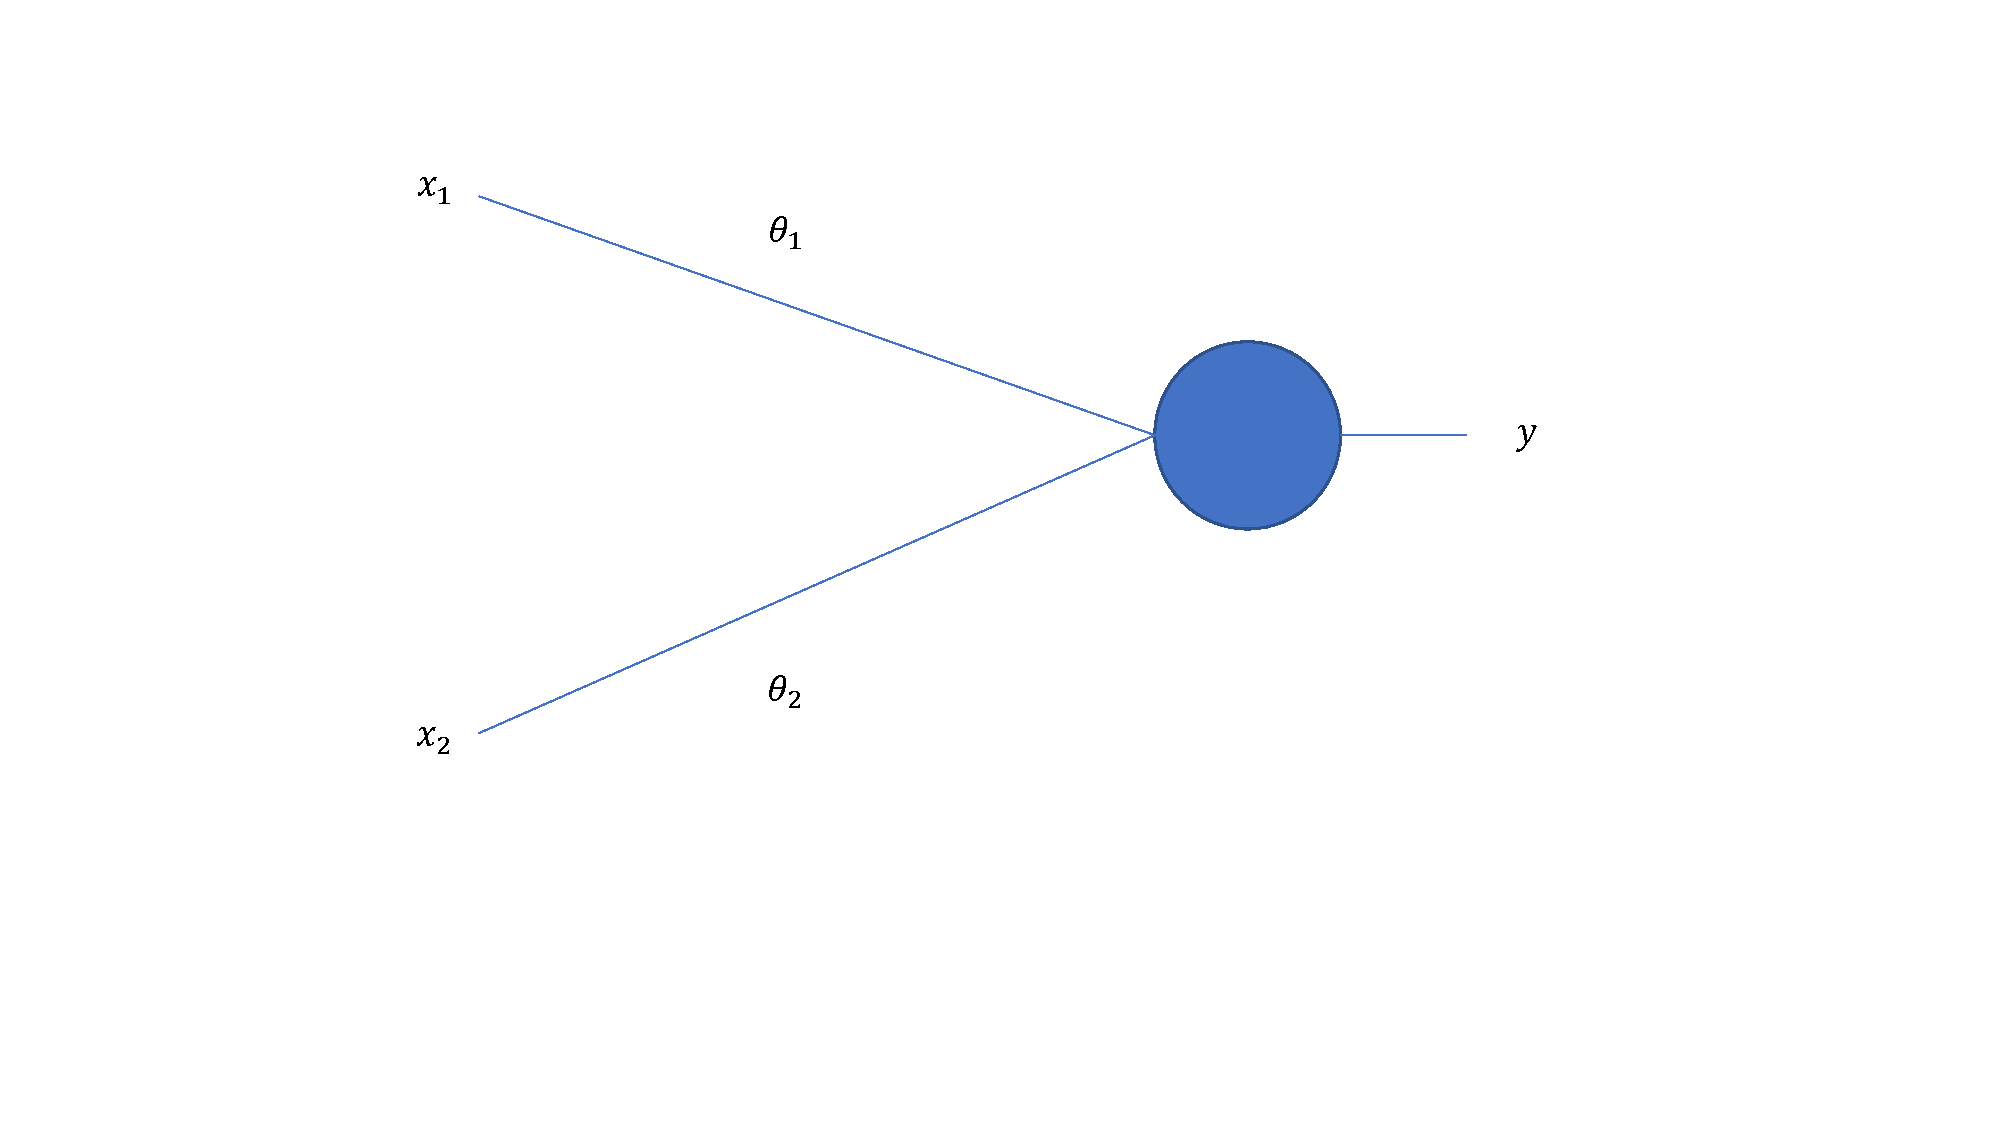
\includegraphics[scale = .3]{perceptron.pdf}}
    
\end{frame}

\begin{frame}
    \frametitle{Sigmoid Activation}

        \begin{itemize}[<+->]
            \item $g(z) = \frac{1}{1+e^{-z}}$
            \item $g'(z) = (1-g(z))g(z)$
        \end{itemize}
    
\end{frame}

\begin{frame}
    \frametitle{Basic Network}

    \centerline{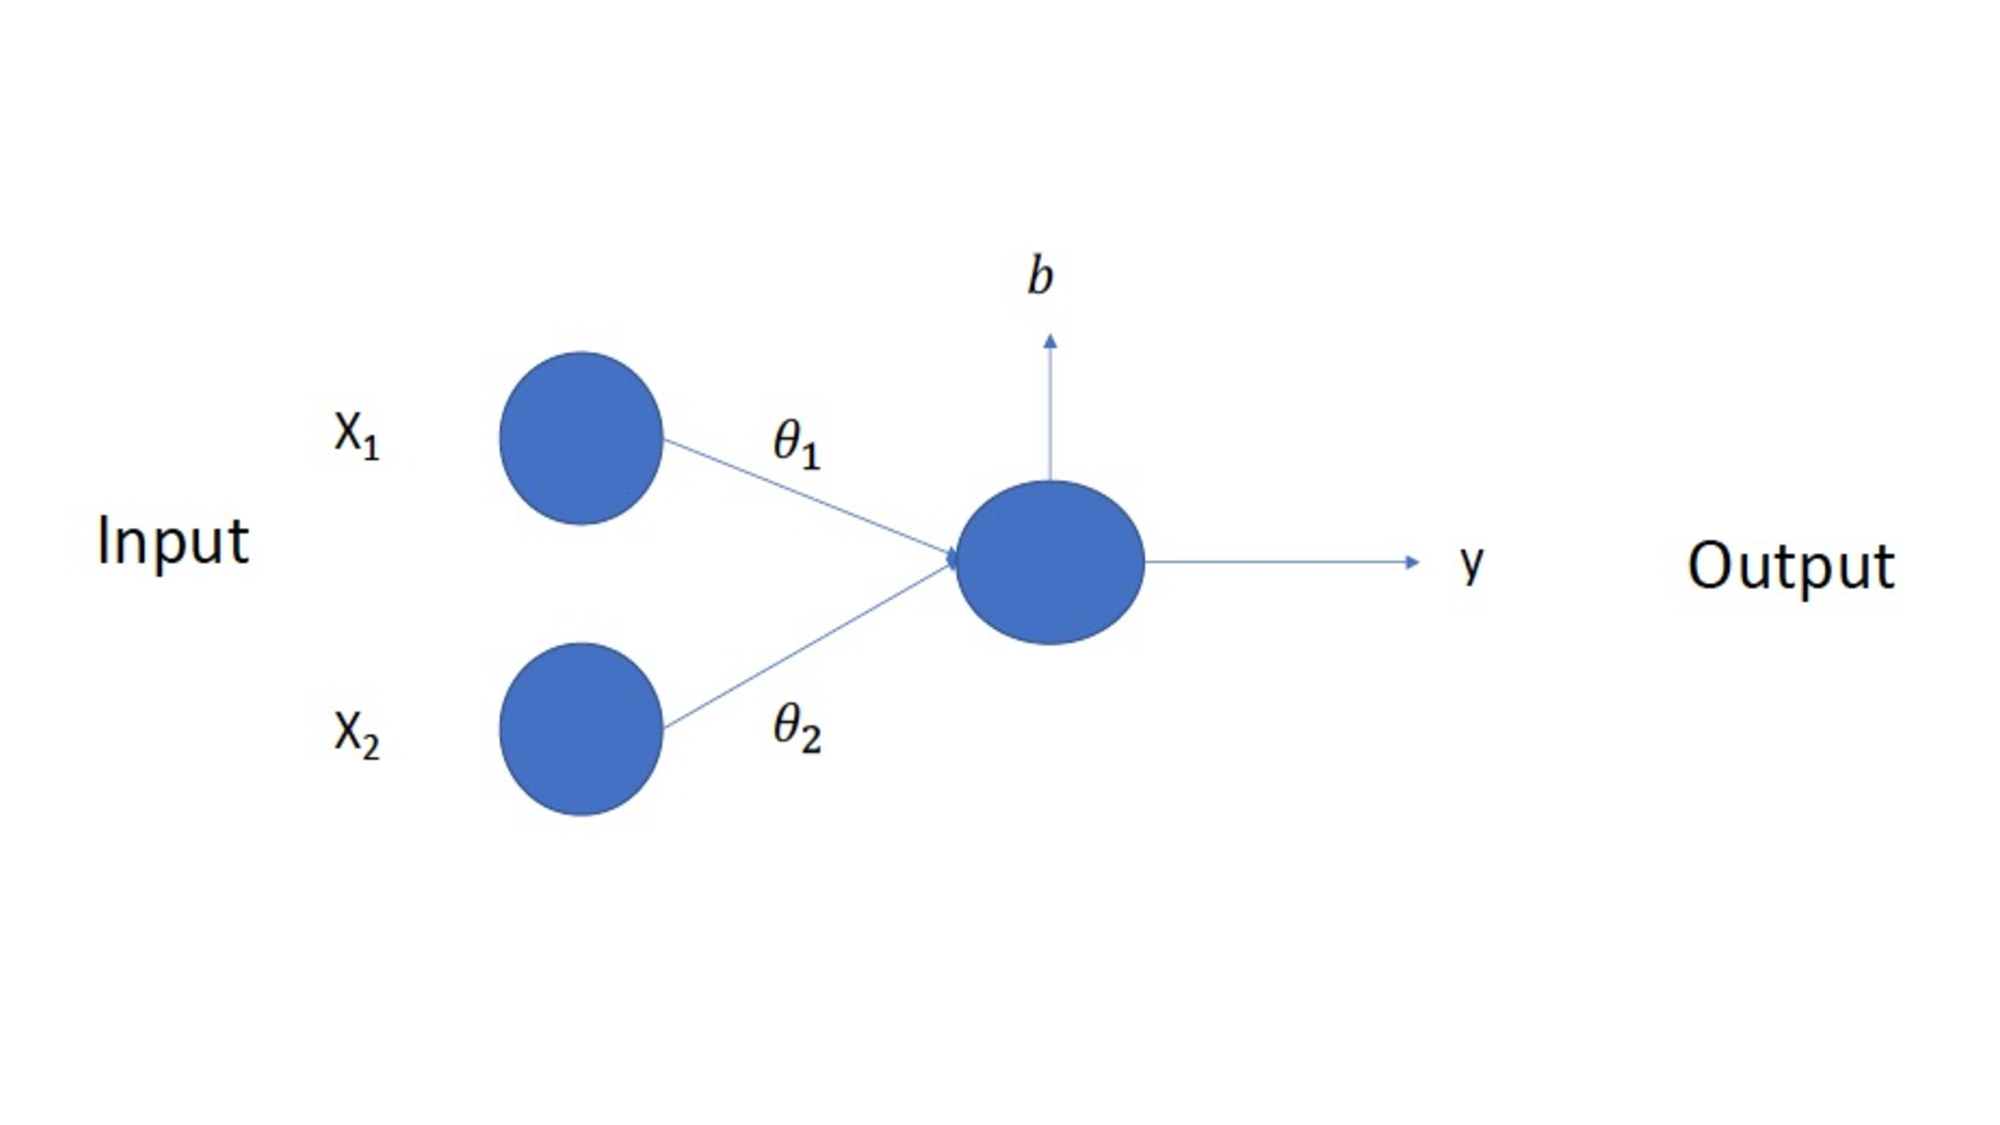
\includegraphics[scale = .3]{FIG1.pdf}}

\end{frame}

\begin{frame}
    \frametitle{Forward Pass}
    Dot Product: 
    \begin{align*}
        z_{k}^{(i)} = \theta_{0} x_0^{(i)} + \theta_{1}x_1^{(i)} + \theta_{2}x_2^{(i)} + \cdots + \theta_{j}x_j^{(i)}
    \end{align*}
    Applying the activation function: 
    \begin{align*}
        a_{k}^{(i)} = g(z_k^{(i)})
    \end{align*}
    
\end{frame}

\begin{frame}
    \frametitle{Loss Function}
    \begin{itemize}[<+->]
        \item Mean Squared Error: 
        \begin{align*}
            J(\theta) = \frac{1}{2m}\sum_{i = 1}^m (a^{(i)} - y^{(i)})^2
        \end{align*}
    \end{itemize}
    
\end{frame}

\begin{frame}
    \frametitle{Gradient Descent}
    Gradient descent iteration: 
    \begin{align*}
        \theta_{n} = \theta_{n-1} - \alpha \frac{\partial J(\theta)}{\partial \theta_{n-1}}
    \end{align*}
    
\end{frame}

\begin{frame}
    \frametitle{Loss Function Derivative}
    \begin{itemize}
        \item Derivative: 
        \begin{itemize}[<+->]
            \item 
            \begin{align*}
                \frac{\partial}{\partial \theta_j} \left( \frac{1}{2m} \sum_{i=1}^m (a^{(i)} - y^{(i)})^2 \right)
            \end{align*}
            \item 
            \begin{align*}
                \frac{1}{2m} \sum_{i=1}^m \frac{\partial}{\partial \theta_j} (a^{(i)} - y^{(i)})^2 
            \end{align*}
            \item 
            \begin{align*}
                \frac{1}{m} \sum_{i=1}^m  (a^{(i)} - y^{(i)}) \frac{\partial}{\partial \theta_j} (a^{(i)})
            \end{align*}
            \item 
            \begin{align*}
                \frac{1}{m} \sum_{i=1}^m  (a^{(i)} - y^{(i)}) g'(z) \frac{\partial}{\partial \theta_j} z
            \end{align*}
        \end{itemize}
        
    \end{itemize}
    
\end{frame}

\begin{frame}
    \frametitle{Loss Function Derivative}

    \begin{align*}
        \frac{\partial J(\theta)}{\partial \theta_{j}} = \frac{1}{m} \sum_{i=1}^m (a^{(i)} - y^{(i)})(1-g(z))(g(z))x_j
    \end{align*}

\end{frame}

\begin{frame}
    \frametitle{Gradient Descent Updates}

        \begin{align*}
            \begin{bmatrix}
                \theta_0 \\
                \theta_1 \\
                \theta_2 
            \end{bmatrix} = 
            \begin{bmatrix}
                \theta_0\\
                \theta_1\\
                \theta_2
            \end{bmatrix} - 
            \alpha
            \begin{bmatrix}
                \frac{1}{m} \sum_{i=1}^m (a^{(i)} - y^{(i)})(1-g(z))(g(z))x_0\\
                \frac{1}{m} \sum_{i=1}^m (a^{(i)} - y^{(i)})(1-g(z))(g(z))x_1\\
                \frac{1}{m} \sum_{i=1}^m (a^{(i)} - y^{(i)})(1-g(z))(g(z))x_2
            \end{bmatrix}
        \end{align*}

\end{frame}

\begin{frame}
    \frametitle{Stochastic Gradient Descent}

    \begin{itemize}
        \item Stochastic Gradient Descent
        \begin{itemize}[<+->]
            \item Small subsets of data
            \item Estimation of gradient 
            \item Quicker compute times
        \end{itemize}
    \end{itemize}

\end{frame}

\begin{frame}
    \frametitle{More Complicated Example}
    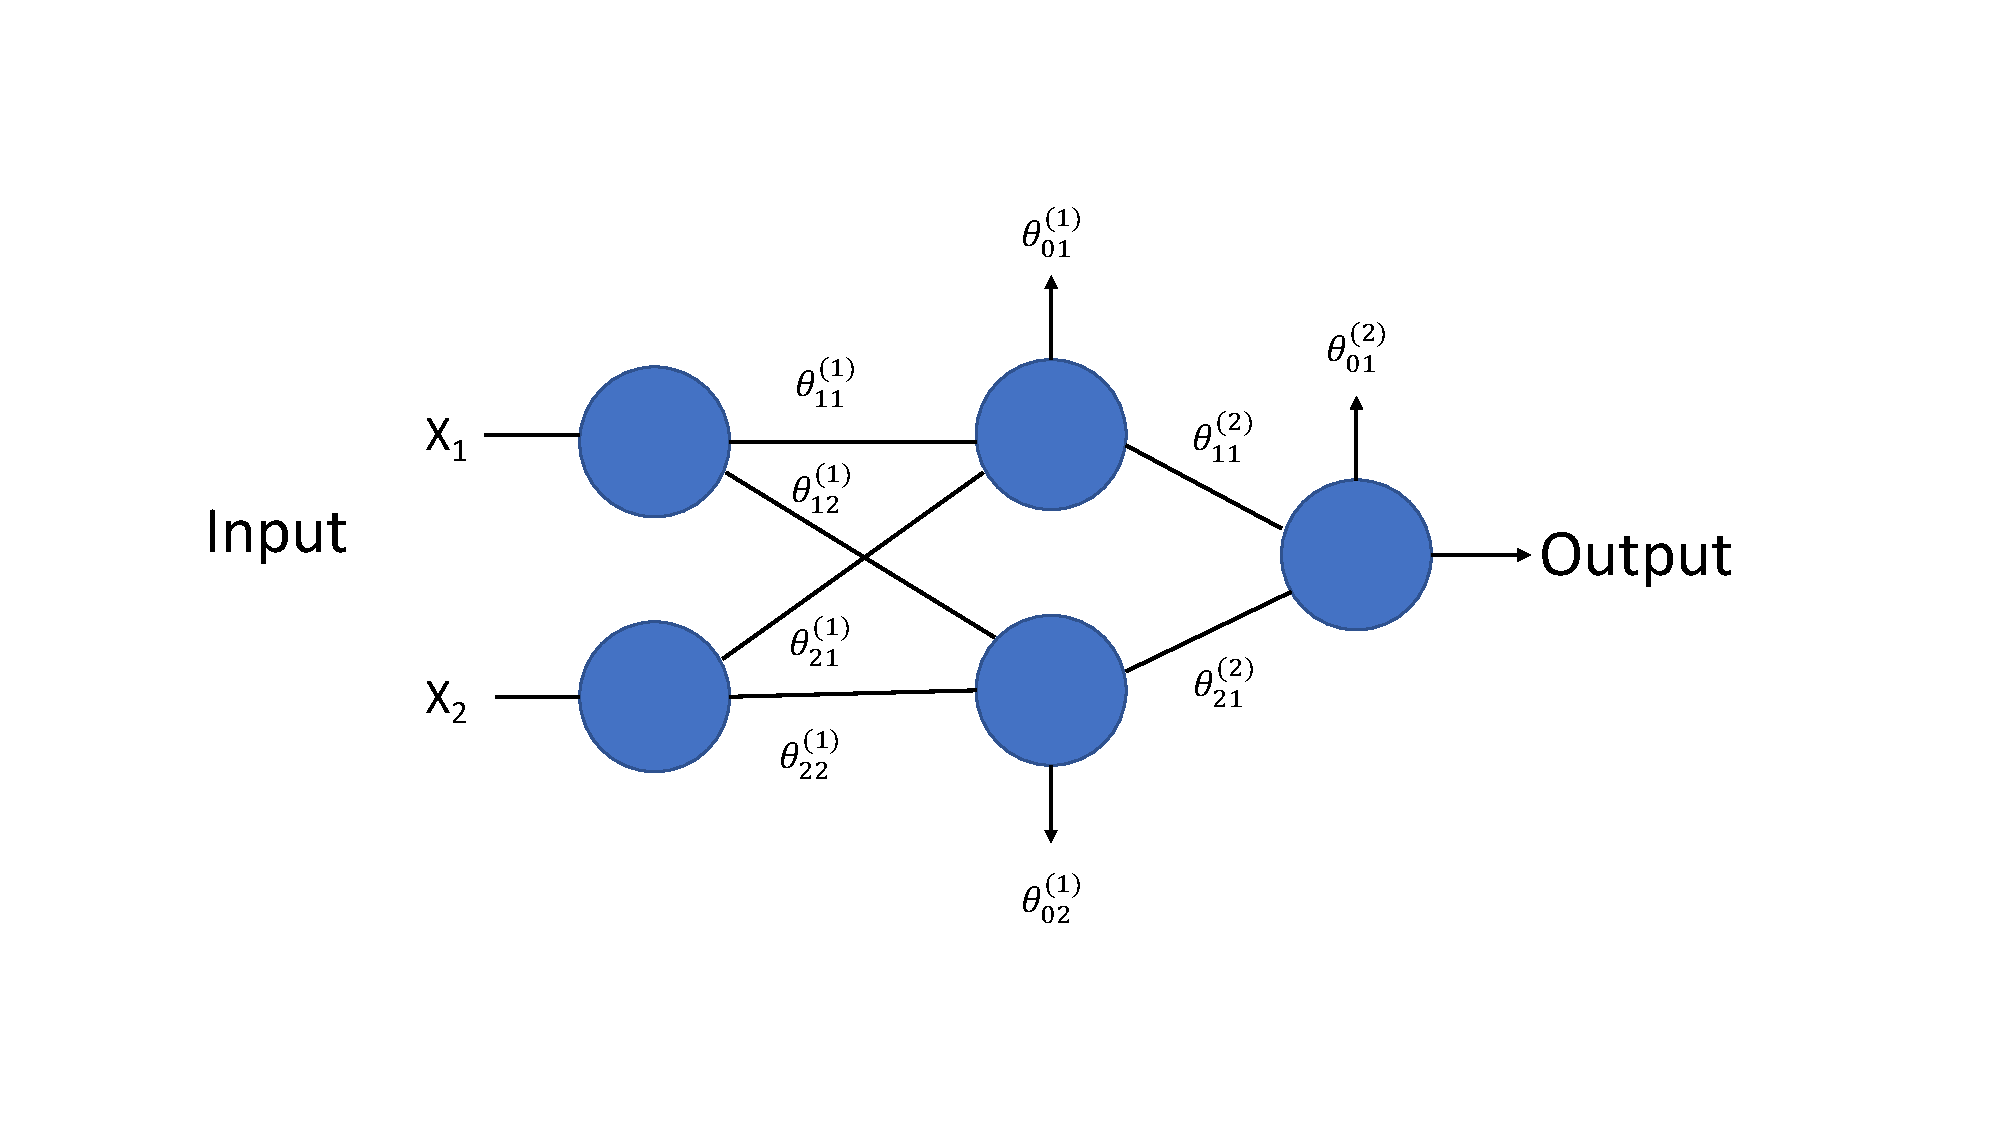
\includegraphics[scale = .3]{FIG2.pdf}\\
\end{frame}

\begin{frame}
    \frametitle{Forward Pass}

    \begin{gather*}
        z^l = (\theta^l)^T a^{l-1}\\
        a^l = g(z^l)\\
        x = a^1
    \end{gather*}

\end{frame}

\begin{frame}
    \frametitle{Back Propagation}

    \centerline{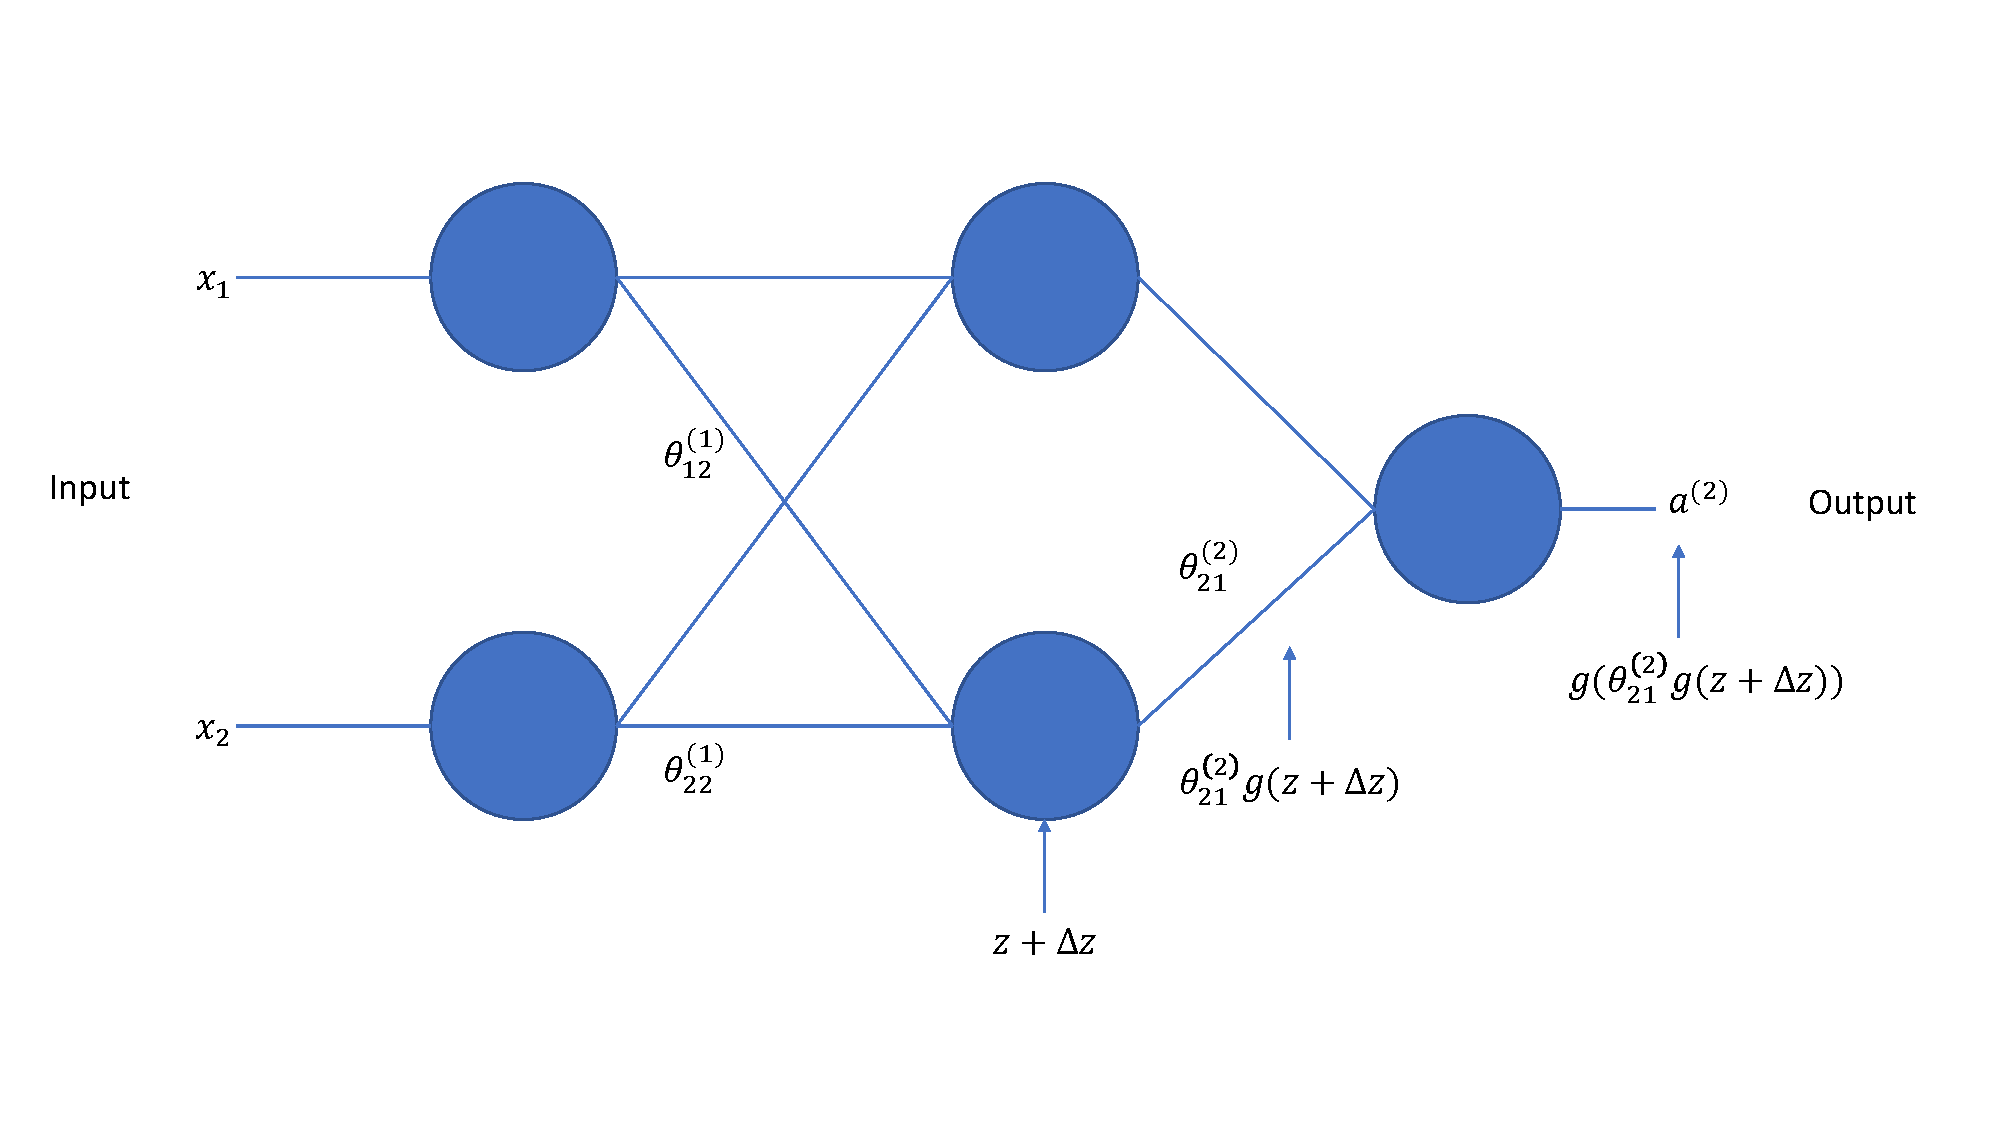
\includegraphics[scale = .3]{backpropintuition.pdf}}

\end{frame}

\begin{frame}
    \frametitle{Back Propagation}

    \begin{gather*}
        \delta^l_j \equiv \frac{\partial J}{\partial z^{l}_j}\\
    \end{gather*}

\end{frame}

\begin{frame}
    \frametitle{First Equation}

    \begin{itemize}[<+->]
        \item 
        \begin{gather*}
            \frac{\partial J}{\partial z^L_j}
        \end{gather*}
        \item 
        \begin{gather*}
            \frac{\partial J}{\partial a_j^L} \frac{\partial a_j^L}{\partial z_j^L}    
        \end{gather*}
        \item 
        \begin{gather*}
            \frac{1}{m}\sum_{j=1}^m(a_j^L - y)g'(z_j^L)
        \end{gather*}
        \item 
        \begin{gather*}
            \nabla_a J \odot g'(z)
        \end{gather*}
    \end{itemize}

\end{frame}

\begin{frame}
    \frametitle{Second Equation}

    \begin{itemize}[<+->]
        \item 
        \begin{gather*}
            \frac{\partial J}{\partial z^l_j}
        \end{gather*}
        \item 
        \begin{gather*}
            \sum_k\frac{\partial J}{\partial z_k^{l+1}} \frac{\partial z_k^{l+1}}{\partial z_j^{l}}    
        \end{gather*}
        \item 
        \begin{gather*}
            \sum_k\delta_k^{l+1}\frac{\partial z_k^{l+1}}{\partial z_j^{l}}
        \end{gather*}
        
    \end{itemize}

\end{frame}

\begin{frame}
    \frametitle{Second Equation}

    \begin{itemize}[<+->]
        \item Since:
        \begin{gather*}
            z_k^{l+1} = \theta_{jk}^{l}\cdot g(z_j^{l}) + \theta_{0k}^{l}
        \end{gather*}
        \item 
        \begin{gather*}
            \sum_k\delta_k^{l+1}\theta_{jk}^{l}g'(z_j^{l})
        \end{gather*}
        \item 
        \begin{gather*}
            (\theta^{l})^T\delta^{l+1} \odot g'(z^{l})
        \end{gather*}
    \end{itemize}

\end{frame}

\begin{frame}
    \frametitle{Third and Fourth Equations}

    \begin{itemize}[<+->]
        \item 
        \begin{gather*}
            \frac{\partial J}{\partial \theta_{jk}^{l}}
        \end{gather*}
        \item 
        \begin{gather*}
            \frac{\partial J}{\partial z_k^{l}}\frac{\partial z_k^{l}}{\partial \theta_{jk}^{l}}
        \end{gather*}
        \item Since:
        \begin{gather*}
            z_k^{l} = \theta_{jk}^{l}\cdot g(z_j^{l-1}) + \theta_{0k}^{l}
        \end{gather*}
        \item 
        \begin{gather*}
            \delta_k^l g(z_j^{l-1}) = \delta_k^l a_j^{l-1}
        \end{gather*}
        
    \end{itemize}
    
\end{frame}

\begin{frame}
    \frametitle{Third and Fourth Equations}

    \begin{itemize}[<+->]
        \item 
        \begin{gather*}
            \frac{\partial J}{\partial \theta_{0k}^{l}}
        \end{gather*}
        \item 
        \begin{gather*}
            \frac{\partial J}{\partial z_k^{l}}\frac{\partial z_k^{l}}{\partial \theta_{0k}^{l}}
        \end{gather*}
        \item Since:
        \begin{gather*}
            z_k^{l} = \theta_{jk}^{l}\cdot g(z_j^{l-1}) + \theta_{0k}^{l}
        \end{gather*}
        \item 
        \begin{gather*}
            \delta_k^l
        \end{gather*}
        
    \end{itemize}
    
\end{frame}

\begin{frame}
    \frametitle{Back Propagation Equations}

    \begin{gather*}
        \delta^l_j \equiv \frac{\partial J}{\partial z^{l}_j}\\
        \delta^L = \nabla_a J \odot g'(z^L)\\
        \delta^{l} = (\theta^{{l}})^T\delta^{l+1} \odot g'(z^{l})\\
        \frac{\partial J }{\partial \theta^l_{jk}} = \delta_k^l a^{l-1}_j \\
        \frac{\partial J }{\partial \theta^l_{0k}} = \delta^l_k
    \end{gather*}

\end{frame}

\begin{frame}
    \frametitle{Mini Batch Code}

    \centerline{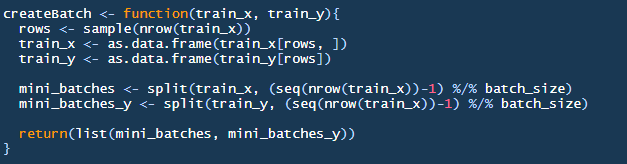
\includegraphics[scale = .6]{createbatch.png}}

\end{frame}

\begin{frame}
    \frametitle{Feed Forward Code}

    \centerline{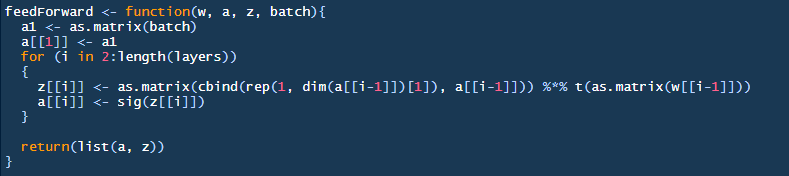
\includegraphics[scale = .5]{feedforward.png}}

\end{frame}

\begin{frame}
    \frametitle{Back Propagation Code}

    \centerline{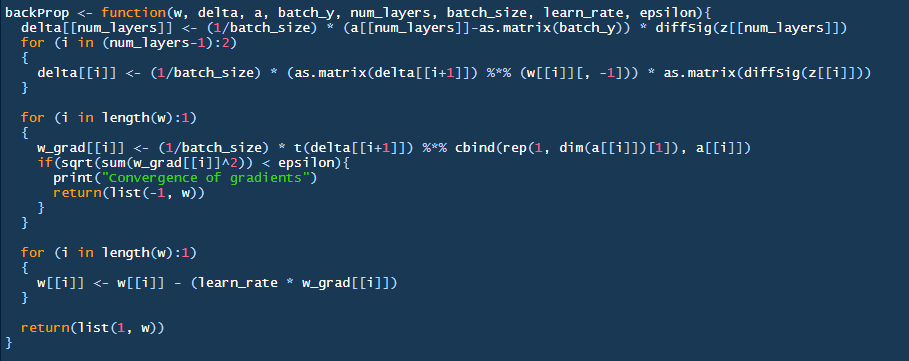
\includegraphics[scale = .43]{backprop.png}}

\end{frame}

\begin{frame}
    \frametitle{Iris Data}

    \centerline{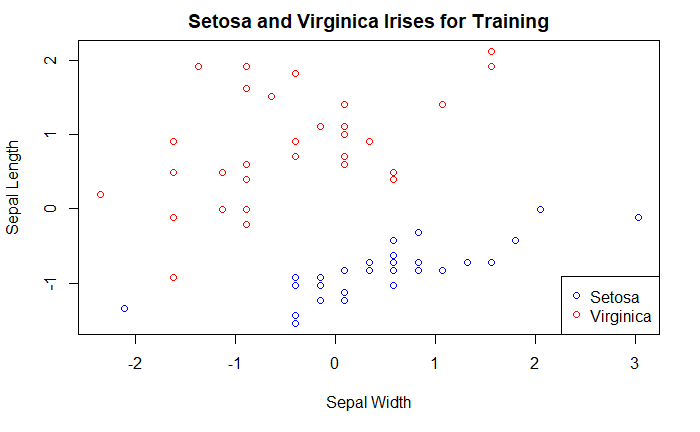
\includegraphics[scale = .5]{irisgraph.png}}

\end{frame}

\begin{frame}
    \frametitle{Simple ANN Results}

    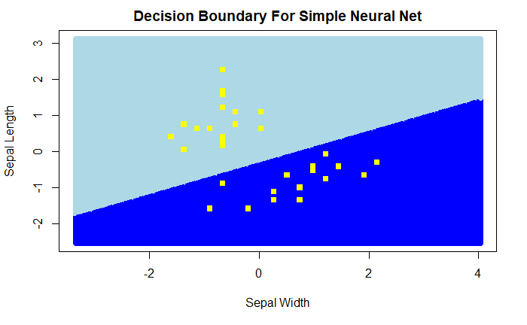
\includegraphics[scale = .69]{irisplane.png}

\end{frame}

\begin{frame}
    \frametitle{Simple ANN Results}

    \centerline{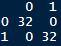
\includegraphics[scale = 2]{simpleconfusionmatrix.png}}

\end{frame}

\begin{frame}
    \frametitle{More Complicated ANN Results}

    \centerline{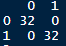
\includegraphics[scale = 2]{nnconfusionmatrix.png}}

\end{frame}

\begin{frame}
    \frametitle{Simple ANN Nonlinear Results}

    \centerline{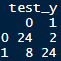
\includegraphics[scale = 2]{simplennnonlinear.png}}

\end{frame}

\begin{frame}
    \frametitle{Complex ANN Nonlinear Results}

    \centerline{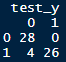
\includegraphics[scale = 2]{complexnnnonlinear.png}}

\end{frame}

\begin{frame}
    \frametitle{}
    \footnotesize
    \setlength{\arraycolsep}{2.5pt}
    \medmuskip = 1mu % default: 4mu plus 2mu minus 4mu
    \begin{itemize}
        \item Normalized data: [Sepal Width, Sepal Length] = 
        $\begin{bmatrix}
            0.5067965 & -0.6560779\\
            -0.6683838 & 0.1603746
        \end{bmatrix}$
        \item Classification: Setosa = $0$, Virginica $1$
    \end{itemize}

    \[
    \scalemath{0.8}{
    \begin{bmatrix}
        1 & 0.5067965 & -0.6560779\\
        1 & -0.6683838 & 0.1603746
    \end{bmatrix}
    \begin{bmatrix}
        -0.2148802 & 2.7147823\\
        1.3172717 & 0.7104345\\
        -2.5719430 & 0.4118125
    \end{bmatrix}= 
    \begin{bmatrix}
        2.140104 & 2.804647\\
        -1.507798 & 2.305984
    \end{bmatrix}
    }
    \]

    \[
    \scalemath{0.8}{
    g \left( \begin{bmatrix}
        2.140104 & 2.804647\\
        -1.507798 & 2.305984
    \end{bmatrix} \right) =
    \begin{bmatrix}
        0.8947404 & 0.9429264\\
        0.1812654 & 0.9093714
    \end{bmatrix}
    }
    \]

    \[
        \begin{bmatrix}
            1 & 0.8947404 & 0.9429264\\
            1 & 0.1812654 & 0.9093714
        \end{bmatrix}
        \begin{bmatrix}
            2.072452\\
            -6.001327\\
            1.215538
        \end{bmatrix}=
        \begin{bmatrix}
            -2.151015\\
            2.089994
        \end{bmatrix}
    \]
    
    \[
        g\left( 
        \begin{bmatrix}
            -2.151015\\
            2.089994
        \end{bmatrix}
        \right) = 
        \begin{bmatrix}
            0.1042364\\
            0.8899269
        \end{bmatrix}
    \]

\end{frame}

\begin{frame}
    \frametitle{References}

    \begin{itemize}
        \item Michael A. Nielsen, “Neural Networks and Deep Learning”, Determination Press, 2015
        \item Rosenblatt, Frank. “The perceptron: a probabilistic model for information storage and organization in the brain.” Psychological review 65.6 (1958): 386.
        \item R. A. Fisher (1936). “The use of multiple measurements in taxonomic problems”. Annals of Eugenics. 7(2): 179-188. 
    \end{itemize}

\end{frame}

\end{document}